\begin{table*}[t!]
\centering
\footnotesize
    \caption{
    Overall experiment results on six tasks. {\bf Bold} numbers indicate the best performance among non-proprietary models, and \textcolor{gray}{\bf gray-colored} bold text indicates the best proprietary model when they outperforms all non-proprietary models.  
    $^*$ indicates concurrent or recent results reported by concurrent work.  -- indicates numbers that are not reported by the original papers or are not applicable. Models are sorted based on scale. FS, em, rg, mau, prec, rec denote FactScore (factuality); str-em, rouge (correctness); MAUVE (fluency); citation precision and recall, respectively. 
    }
    \label{tab:main}
\begin{tabular}{lrrrrrrrrrr}\toprule
&\multicolumn{2}{c}{Short-form} & \multicolumn{2}{c}{Closed-set} & \multicolumn{6}{c}{Long-form generations (with citations)}     \\
& PopQA & TQA &  Pub & ARC &  Bio  &\multicolumn{5}{c}{ASQA} \\ 
LM & (acc) & (acc) & (acc) & (acc) & (FS) & (em) & (rg) & (mau) & (pre) & (rec) \\
\midrule
\multicolumn{11}{c}{\it LMs with proprietary data } \\
Llama2-c$_{\textsc{13b}}$  & 20.0 & 59.3 & 49.4 & 38.4 & 55.9 & 22.4 & 29.6 & 28.6 & -- & -- \\
Ret-Llama2-c$_{\textsc{13b}}$  & 51.8  & 59.8& 52.1 & 37.9 &  {79.9} & 32.8 & 34.8 & 43.8 & 19.8& 36.1 \\
ChatGPT  & 29.3 &   \textcolor{gray}{\bf 74.3} & 70.1 &  \textcolor{gray}{\bf 75.3}  & 71.8 & 35.3  & 36.2  & 68.8 & -- & --\\ 
Ret-ChatGPT &  50.8 & 65.7 &  54.7 & \textcolor{gray}{\bf 75.3} & -- & \textcolor{gray}{\bf 40.7} &  \textcolor{gray}{\bf 39.9} & \textcolor{gray}{\bf 79.7} & {65.1} & \textcolor{gray}{\bf 76.6}  \\
Perplexity.ai &  -- & -- & -- & -- & 71.2 & -- &  -- & -- & -- &--  \\ \midrule
\multicolumn{11}{c}{\it Baselines without retrieval} \\
Llama2$_{\textsc{7b}}$ & 14.7 & 30.5 & 34.2 & 21.8  & 44.5  & 7.9 & 15.3&19.0 & -- & --  \\
Alpaca$_{\textsc{7b}}$  &  23.6 & 54.5  & 49.8 &45.0 & 45.8 & 18.8 & 29.4 & 61.7 & -- & --  \\
Llama2$_{\textsc{13b}}$   &  14.7 & 38.5  & 29.4 & 29.4 & 53.4 & 7.2 & 12.4 & 16.0  & -- & -- \\
Alpaca$_{\textsc{13b}}$ &  24.4  &  61.3  & 55.5  & 54.9 & 50.2 & 22.9 &  32.0&  70.6 & -- & -- \\
CoVE$_{\textsc{65b}}$ * &  -- & -- & -- & -- & 71.2  & --  & -- & -- & -- & -- \\  
\midrule

\multicolumn{11}{c}{\it Baselines with retrieval} \\
Toolformer*$_{\textsc{6b}}$  & -- & 48.8  & -- & -- & -- & --  & -- & -- & -- & --  \\ 
Llama2$_{\textsc{7b}}$  & 38.2  & 42.5 & 30.0 & 48.0 & 78.0 & 15.2 & 22.1 & 32.0 & 2.9 & 4.0 \\
Alpaca$_{\textsc{7b}}$   & 46.7 & 64.1  & 40.2 & 48.0 & 76.6  & 30.9 & 33.3 & 57.9 & 5.5 & 7.2 \\
Llama2-FT$_{\textsc{7b}}$  & 48.7 & 57.3 & 64.3 & 65.8& {78.2} & 31.0 & 35.8 & 51.2 & 5.0 & 7.5 \\
SAIL*$_{\textsc{7b}}$  &  -- & -- & 69.2 & 48.4 & -- & --  & -- & -- & -- & --  \\ 
Llama2$_{\textsc{13b}}$  &  45.7  & 47.0 & 30.2  & 26.0 & 77.5  & 16.3 & 20.5 & 24.7 & 2.3 & 3.6  \\
Alpaca$_{\textsc{13b}}$ & 46.1& {66.9}  &  51.1 & 57.6 & 77.7 & {\bf 34.8} & 36.7 & 56.6 & 2.0 & 3.8 \\
\hdashline
{\bf Our }\model$_{\textsc{7b}}$ &{  54.9} &  66.4  & { 72.4} & 67.3 & {\bf 81.2} & 30.0 & 35.7 & {\bf 74.3} & {66.9} & { 67.8} \\
{\bf Our }\model$_{\textsc{13b}}$  &  {\bf 55.8} & {\bf 69.3} & {\bf 74.5} & {\bf 73.1} &  80.2 & 31.7 & {\bf 37.0} & { 71.6} & {\bf 70.3} & {\bf 71.3} \\
\bottomrule
\end{tabular}
\end{table*}


\subsection{Main Results} 
\noindent{\bf Comparison against baselines without retrieval. }
Table~\ref{tab:main} (top) presents the baselines without retrieval. 
Our \model (bottom two rows) demonstrates a substantial performance advantage over supervised fine-tuned LLMs in all tasks and even outperforms ChatGPT in PubHealth, PopQA, biography generations, and ASQA (Rouge and MAUVE). 
Our approach also significantly outperforms a concurrent method that employs sophisticated prompt engineering; specifically, on the bio generation task, our 7B and 13B models outperform the concurrent CoVE~\citep{dhuliawala2023chainofverification}, which iteratively prompts Llama2$_\textsc{65b}$ to refine output. 

\noindent{\bf Comparison against baselines with retrieval.}
As shown in Tables~\ref{tab:main} (bottom), our \model also outperforms existing RAG in many tasks, obtaining the best performance among non-proprietary LM-based models on all tasks. 
While our method outperforms other baselines, on PopQA or Bio, powerful instruction-tuned LMs with retrieval (e.g., LLama2-chat, Alpaca) show large gains from their non-retrieval baselines. 
However, we found that these baselines provide limited solutions for tasks where we cannot simply copy or extract sub-strings of retrieved passages. 
On PubHealth and ARC-Challenge, baselines with retrieval do not improve performance notably from their no-retrieval counterparts.
% , indicating that simple input augmentation may not immediately improve all knowledge-intensive tasks. 
We also observe that most baselines with retrieval struggle to improve citation accuracy. 
On ASQA, our model shows significantly higher citation precision and recall than all models except ChatGPT. 
\citet{gao2023enabling} found that ChatGPT consistently exhibits superior efficacy in this particular task, surpassing smaller LMs. 
{
Our \model bridges this performance gap, even outperforming ChatGPT in citation precision, which measures whether the model-generated claim is fully supported by cited evidence. } 
We also found that on the metrics for factual precision, \model 7B occasionally outperforms our 13B due to the tendency of smaller \model to often generate precisely grounded yet shorter outputs. 
{
Llama2-FT$_{\textsc{7b}}$, which is the baseline LM trained on the same instruction-output pairs as \model without retrieval or self-reflection and is retrieval-augmented at test time only, lags behind \model. This result indicates \model gains are not solely from training data and demonstrate the effectiveness of \model framework.  } 



\begin{figure}[t!]
\begin{subfigure}[b]{0.38\textwidth}
\centering
\footnotesize
\begin{tabular}{lccc}
\toprule
 & PQA & Med & AS \\
 & (acc) & (acc) & (em) \\
\midrule
\model (50k) & 45.5 & 73.5  & 32.1 \\ \hdashline
\multicolumn{4}{l}{\it Training } \\
No Retriever \mret & 43.6 & 67.8 & 31.0 \\
No Critic \mcrt &  42.6 & 72.0 & 18.1  \\\hdashline
\multicolumn{4}{l}{\it Test } \\
No retrieval & 24.7 &  73.0 & --  \\
Hard constraints&  28.3 &  72.6 & --  \\
Retrieve top1 & 41.8 & 73.1 & 28.6  \\
Remove \cgr & 44.1  & 73.2 & 30.6 \\ 
\bottomrule
\end{tabular}
\caption{ Ablation}
\label{tab:ablatioon}
\end{subfigure}%
  \hspace{.3cm}
  \begin{subfigure}[b]{0.265\textwidth}
        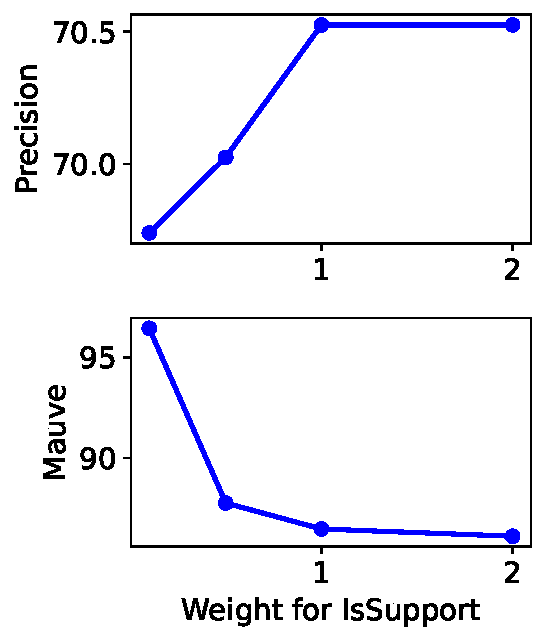
\includegraphics[width=\textwidth]{figs/soft_alignment.pdf}
        \caption{Customization}
        \label{fig:customization}
  \end{subfigure}%
    \begin{subfigure}[b]{0.325\textwidth}
        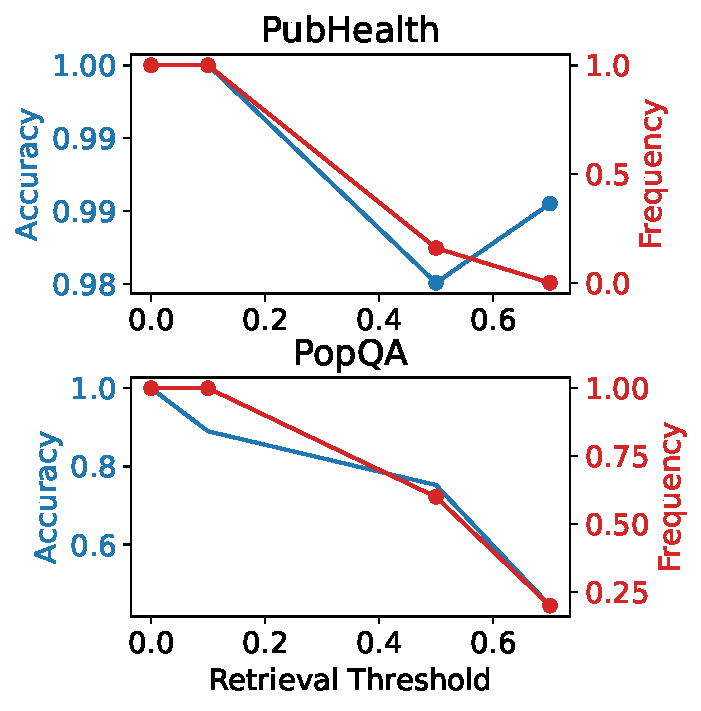
\includegraphics[width=\textwidth]{figs/tradeoff_fever.pdf}
        \caption{Retrieval}
        \label{fig:retrieval_freq}
  \end{subfigure}%
\caption{{\bf Analysis on \model:} (a) {\bf Ablation studies} for key components of \model training and inference based on our 7B model.  (b) {\bf Effects of soft weights} on ASQA citation precision and Mauve (fluency). (c) {\bf Retrieval frequency} and {\it normalized} accuracy on PubHealth and PopQA.   }
\end{figure}
\subsection{Analysis}
\label{sec:analyis}
\paragraph{Ablation studies.}
We conduct a set of ablations of our framework to identify which factors play key roles. 
We evaluate two model variants trained differently than our model: {\it No Retriever} trains an LM using the standard instruction-following method given instruction-output pairs, without retrieved passages;  {\it No Critic} trains an LM trained with input-output pairs that are always augmented with the top one retrieved document without reflection tokens. 
This is similar to SAIL~\citep{luo2023sail}, and we use our instruction-output data instead of using the Alpaca dataset~\citep{dubois2023alpacafarm}, as in SAIL. 
We also conduct ablation on our inference-time algorithm, including {\it No retrieval} disables retrieval during inference; {\it Hard constraints} indicates the model performance that retrieves when \ret=\texttt{Yes} instead of using the adaptive threshold; {\it Retrieve top 1} always retrieves and uses the top one document only, similar to standard RAG approaches; {\it Remove \cgr} indicates the model performance that removes \cgr score only during critique-guided beam search in Eq.~\ref{eq:reward}. 
%\sandy{Below, do you mean Figure 3??? That's what the title shows.} 
{In this ablation experiment, we use a training instance size of 50k for a more efficient exploration of training variations. Later in this section, we conduct an analysis of the effect of training data size. 
We conduct the ablation studies on three datasets, PopQA, PubHealth, and ASQA. On ASQA, we evaluate models on sampled 150 instances and exclude ablations involving adaptive or no retrieval processes. }

We show in Table~\ref{tab:ablatioon} the ablation results. 
The top part of the table shows results for training ablations, and the bottom part is for inference ablations. We see that all components play important roles.
We also observe a large performance gap between \model and No Retriever or Critic baselines across tasks, indicating that training an LM with those models largely contributes to the performance gain of \model. 
{
Using the top passages regardless of their relevance (Retrieve top 1) as in conventional RAG approaches causes a large drop in PopQA and ASQA, and removing \cgr during the beam search results hurts performance on ASQA. 
This demonstrates the effectiveness of \model's capabilities of carefully selecting generations based fine-grained multiple criterion, instead of naively using all of the top passages from the retrieval model or solely depending on relevance scores. 
}


\noindent{\bf Effects of inference-time customization.}
One key benefit of our proposed framework is that it enables us to control how much each critique type affects the final generation sampling. We analyze the effects of different parameter weights on the top of our 7B model during inference time on ASQA, where multiple evaluation aspects are considered. 
Figure~\ref{fig:customization} shows the effects of changing the weighting term for \cgr, which criticizes how supported the output is by the text passage. 
As the figure shows, increasing the weight leads to positive effects on the models' citation precision since this puts more emphasis on whether model generation is supported by the evidence. 
{
On the contrary, a larger weight results in lower MAUVE scores: when generation gets longer and more fluent, there are often more claims that are not fully supported by citations, consistent with findings by \cite{liu2023evaluating}. }
Our framework lets practitioners choose and customize models' behaviors at test time by adjusting such parameters without requiring additional training. 

\noindent{\bf Efficiency and accuracy trade-off.}
% \akari{merge two charts (A) and (B); normalized }
Using our framework, practitioners can adjust how often retrieval occurs using the token probability of reward tokens. We evaluate how this adaptive threshold affects overall accuracy and frequency of retrieval, and we evaluate the performance with varying numbers of threshold $\delta$ (larger $\delta$ results in less retrieval) on PubHealth and PopQA. 
Figure~\ref{fig:retrieval_freq} shows that the model's retrieval frequencies dramatically change on both datasets. as $\delta$ varies.  
On one hand, performance deterioration by retrieving less is smaller on PubHealth but larger in PopQA. 

\noindent{\bf Effects of training data size.}
{We conduct an analysis of how the data scale affects the model's performance. In particular, we randomly sample 5k, 10k, 20k, and 50k instances from our original 150k training instances, and fine-tune four \model$_{\textsc{7b}}$ variants on those subsets. Then, we compare the model performance on PopQA, PubHealth, and ASQA (citation precision) with our final \model trained on the full 150k instances. 
We also evaluate 
Figures~\ref{fig:popqa_scale}, \ref{fig:med_sacle} and \ref{fig:asqa_prec_scaling} shows the models' performance trained on different amount of data. 
Across all datasets, increasing data size often shows upward trajectories and the improvements are significantly larger in PopQA and ASQA, while we do not observed such significant improvements on Llama2-FT$_{\textsc{7b}}$ when increasing the training data from 50k to 150k. 
These results also indicate that further expanding the training data of \model may lead to further improvements, although in this work we limit our training data size to 150k. 
}

\noindent{\bf Human evaluations.}
{We conduct small human evaluations on \model outputs, as well as the reliability of predicted reflection tokens. 
In particular, we sampled 50 samples from PopQA and Bio results. 
Following \citet{menick2022teaching}, human annotators evaluate {\it S\&P}, which indicates whether the model output is plausible (i.e., the output is a reasonable and on-topic response to the question as if it were occurring in a conversation) and supported (i.e., the provided evidence is sufficient to verify
the validity of the answer). For {S\&P}, we do not consider the instances where \model predicts \texttt{irrelevant} or \texttt{no support}. 
We then ask our annotators whether the model-predicted reflection tokens about \crel and \cgr match their inspections (e.g., whether the {\it fully supported} output is supported by the cited evidence).  
% In the Appendix, we provide model predictions. 
Human annotators find \model answers are often plausible and supported by relevant passages with higher S\&P scores on short-form PopQA, which is consistent with \citet{menick2022teaching}. 
Human annotators also find \crel and \cgr reflection token predictions are mostly aligned with their assessments. 
Appendix Table~\ref{tab:human_evaluations} shows several annotated examples and explanations on assessments. 
}

\begin{figure}[t!]
  \begin{subfigure}[b]{0.24\textwidth}
        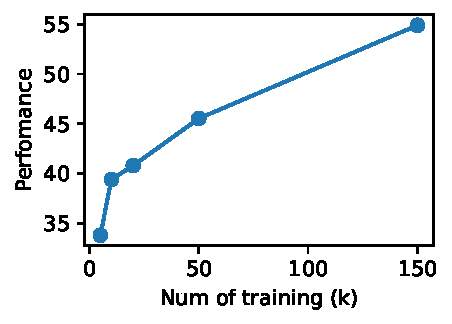
\includegraphics[width=\textwidth]{figs/PopQA_scale.pdf}
        \caption{PopQA}
        \label{fig:popqa_scale}
  \end{subfigure}%
    \begin{subfigure}[b]{0.21\textwidth}
        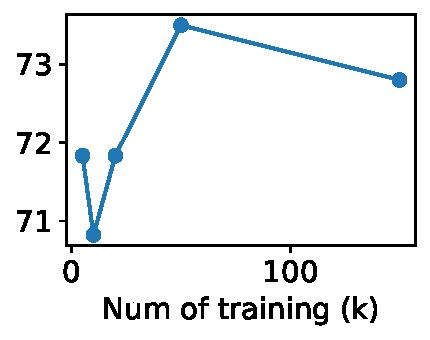
\includegraphics[width=\textwidth]{figs/med_scale.pdf}
        \caption{PubHealth}
        \label{fig:med_sacle}
  \end{subfigure}%
    \begin{subfigure}[b]{0.21\textwidth}
        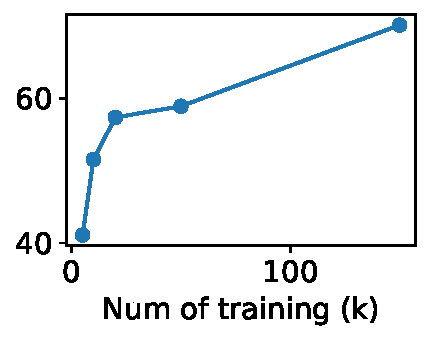
\includegraphics[width=\textwidth]{figs/ASQA_Prec.pdf}
        \caption{ASQA (prec)}
        \label{fig:asqa_prec_scaling}
  \end{subfigure}
\begin{subfigure}[b]{0.3\textwidth}
\centering
\footnotesize
\begin{tabular}{lcc}
\toprule
& Pop & Bio. \\
\midrule
S \& P & 92.5 & 70.0 \\ \hdashline
\crel & 95.0 & 90.0 \\
\cgr & 90.0 &  85.0 \\
\bottomrule
\end{tabular}
\caption{Human evaluation on PopQA and Bio generation. }
\label{tab:human_eval}
\end{subfigure}%
  \hspace{.3cm}
\caption{{\bf Training scale and Human analysis:} (a) (b) (c) {\bf Training scale analysis} shows the effect of the training data scale on PopQA, PubHealth and ASQA (citation precision), respectively.  
(d) {\bf Human analysis} on \model outputs as well as reflection tokens. }
\end{figure}